%----------------------------------------------------------------------
\documentclass{article}

\usepackage[homework]{brownpreamble}
\lhead{\color{light-gray} \itshape Math Camp 2021}
\rhead{\color{light-gray} \itshape Suggested Solutions 1}
\renewcommand\sectiontype{Suggested Solutions \thesection\ }
% \renewcommand\thesection{\arabic{section}}
% \setcounter{section}{0}

%----------------------------------------------------------------------
\begin{document}
\displayoptions

\textbf{\textit{General Strategy for Proofs:}} Before delving into the solutions, I wanted to give a simple algorithm for how to approach proofs \textit{when you don't know where to start}. If you have an idea of what to do, go for it! However, if you are struggling or a bit lost, this  is a simple algorithm I like to follow to get going:
\begin{enumerate}
  \item \textbf{\textit{List}} the assumptions given by the problem. (\textit{Literally} make a bullet list.)

  \item State what you \textbf{\textit{WTS}} (want to show) and what it \textit{\textbf{means}}. (Often what you are asked to show should be stated precisely so that your goal is clear.)

  \item Start walking through the \textit{\textbf{implications}} of the list of assumptions.
\end{enumerate}

Spelling out every detail can take a long time, so I don't necessarily recommend this if you already know where to start. However, when I am lost I find this structured way of approaching problems helps. (Though keep in mind that  this is just my personal suggestion; if you are looking for something more polished, my math professor recommended \textit{How to Solve It} by G. Polya. I haven't read it but I hear good things.) In this set of solutions, I solve the last problem in tedious detail following the algorithm above.

% ---------------------------------------------------------------------
\clearpage
\section{}

\begin{enumerate}[1.]
  \item \textit{Show, by induction, the Bernoulli inequaliity: If $x > -1 \implies (1 + x)^n \ge 1 + nx ~ \forall n \in \mathbb{N}$}

    \solution The base case is $n = 1$. So we have
    \begin{align*}
        1 + x & \ge 1 + x
    \end{align*}

    which holds with equality, so the base case is true. Now the inductive step:
    \begin{align*}
        (1 + x)^n & \ge 1 + nx
    \end{align*}

    If $x > -1$, then the $\log(1 + x)$ is defined for all $x$. Hence
    \begin{align*}
        n \log(1 + x)               & \ge \log(1 + nx)                          \\
        n \log(1 + x) + \log(1 + x) & \ge \log(1 + nx) + \log(1 + x)            \\
        (n + 1) \log(1 + x)         & \ge \log((1 + nx)(1 + x))                 \\
        (1 + x)^{n + 1}             & \ge (1 + nx) (1 + x) =  1 + nx + x + nx^2 \\
                                    & =   1 + nx + x + nx^2                     \\
                                    & \ge 1 + nx + x                            \\
                                    & =   1 + (n + 1)x                          \\
        (1 + x)^{n + 1}             & \ge 1 + (n + 1)x
    \end{align*}

  \item \textit{Show, by contradiction, that the set of prime numbers of infinite.}

    \solution Suppose not, that is, that the finite set $\mathcal{P} =
      \set{p_1, \ldots, p_N}$ contains all prime numbers. Define
      \[
          \widetilde{p}_N = 1 + \prod_{i = 1}^N p_i
      \]

      Note $\widetilde{p}_N > p_i$ for any $i$, so $\widetilde{p}_N \notin \mathcal{P}$. Further, since $p_i$ is prime for all $i$, $\widetilde{p}_N$ cannot be divided by any $p_i$. Hence $\widetilde{p}_N$ is prime and not in the set of all primes, a contradiction. Now we only need to show that the product of $N$ primes plus 1 is not divisible by any of them. Suppose that it is, then we can write
      \[
          1 + \prod_{i = 1}^N p_i = p_j * K
      \]

      for some $j \le N$ and some $K \in \mathbb{N}$ (since $p_i > 1$ for all $i$). However, note that
      \[
          p_j * K
          = 1 + \prod_{i = 1}^N p_i
          = 1 + p_j * \prod_{i = 1, i \ne j}^N p_i
          > p_j * \prod_{i = 1, i \ne j}^N p_i
      \]

      Which means that $K > \prod_{i = 1, i \ne j}^N p_i$ and hence $K \ge \prod_{i = 1, i \ne j}^N p_i + 1$ (since $K \in \mathbb{N}$). Last,
      \[
          p_j * K
          \ge p_j * (\prod_{i = 1, i \ne j}^N p_i + 1)
          = p_j * \prod_{i = 1, i \ne j}^N p_i + p_j
          = pj + \prod_{i = 1}^N p_i
          > 1 + \prod_{i = 1}^N p_i
      \]

      gives the contradiction $p_j * K > 1 + \prod_{i = 1}^N p_i$, which was supposed to hold with equality.

  \item \textit{Show the supremum of a set of real numbers is unique.}

    \solution Take a set $S \subseteq \mathbb{R}$. If it is not bounded above, the supremum does not exist.\footnote{Suppose the supremum $\sup S$ is finite; then since $S$ is not bounded, $\exists \widetilde{s} \in S$ that is greater than $\sup S$, which means $\sup S$ is not greater than every element in $S$, a contradiction.} Hence $S$ is bounded above: Take a supremum of the set and call it $s$, and by contradiction suppose $\widetilde{s} \ne s$ is also a supremum of $S$.  If $s > \widetilde{s}$ then $s$ is not a supremum because there is a smaller number that also bounds $S$; similarly if $s < \widetilde{s}$ then $\widetilde{s}$ is not a supremum because there is a smaller number that also bounds $S$. Either way we have a contradiction.

  \item \textit{Let $A$ and $B$ be non-empty real-valued sets bounded above. Let $C = \set{a +b: a \in A, b \in B}$. Show $\sup C = \sup A + \sup B$}

    \solution We have that $\sup C \ge c ~~ \forall c \in C$, hence $\sup C \ge a + b ~~ \forall a \in A, b \in B$.  Since $\sup A \ge a ~~ \forall a \in A$ and $\sup B \ge b ~~ \forall b \in B$, $\sup A + \sup B \ge a + b ~~ \forall a \in A, b \in B$.

      Importantly, $\cancel{\exists} \widetilde{c} \ge c ~~ \forall c \in C$ s.t. $\widetilde{c} < \sup C$, by definition of the supremum. Similarly for $\sup A$ and $\sup B$. Hence it cannot be that $\sup C > \sup A + \sup B$, or $\sup A + \sup B$ would be the supremum of $C$ instead of $\sup C$, a contradiction.

      Now suppose that $\sup C < \sup A + \sup B$, which implies $\sup C - \sup B < \sup A$. By definition of the $\sup$, this implies $\exists a \in A$ s.t. $\sup C - \sup B < a \le \sup A$, or $\sup C - a < \sup B$. Again by definition of the $\sup$, $\exists b \in B$ s.t. $\sup C - a < b \le \sup B$, or $\sup C < a + b$. However, one last time, $a + b \le \sup C$ by definition of the $\sup$, contradiction.

  \item \textit{Given a real sequence $(a_j)$, define}
    \[
        b_m = \sum^{m}_{j = 1} a_j
        \quad\quad
        c_m = \sum^{m}_{j = 1} |a_j|
    \]

    \textit{Show $(b_m)$ converges if $(c_m)$ converges. Give an example of $(a_j)$ to show the converse may not hold.}

      \solution Suppose $c_m \to c$ and define 
      \[
          b_m^+ = \sum^{\infty}_{j: a_j \ge 0} a_j
          \quad\quad
          b_m^- = \sum^{\infty}_{j: a_j < 0} a_j
      \]

      $b_m^+$ is increasing since $b_{m + 1}^+ = b_m^+$ or $b_m^+ + a_{m +1} \ge b_m^+$. Similarly, we have that $b_m^-$ is decreasing. Since $0 \le a_j \le |a_j|$, we further have that
      \[
          0 \le b_m^+ \le c_m \le c
          \quad\quad
          0 \ge b_m^- \ge -c_m \ge -c
      \]

      Since $c_m$ is increasing and $c_m \to c$, we know that $c_m \le c$. Further, we know from class that a bounded increasing sequence converges, and a bounded decreasing sequence also converges. Since $b_m = b_m^+ + b_m^-$ for all $m$, and $b_m^+ \to b^+, b_m^- \to b^-$ for some $b^+, b^-$, it must be that $b_m \to b^+ + b^-$. For the converse, take for instance
      \[
          a_j = \set{-1, 1, -1 / 2, 1 / 2, \ldots, (-1^m) / m}
      \]

      The sum converges to 0. If $m$ is odd, then $b_m = -1 / m$; if $m$ is even, then $b_m = 0$. However, $c_m$ diverges, since it becomes 2 times the sum of the harmonic series, which diverges.

  \item \textit{Show if $(x_m)$ is a bounded and monotonic real sequence then $(x_m)$ converges.}

    \solution Here I want to try something different: The idea is to give you a detailed outline of how I would work through a proof if I wasn't sure where to start, spelling out my reasoning and each step in overly verbose detail.

    % \begin{align*}
    %   \underline{x} = \inf \Fset{x_m}
    %   \quad\text{and}\quad
    %   \overline{x} = \sup \Fset{x_m}
    % \end{align*}
    %
    % exist. If $x_m$ is increasing we claim $x_m \to \overline{x}$. By definition of $\sup$, for any $\varepsilon > 0$ there exists some $M$ s.t.
    % \begin{align*}
    %   \overline{x} - \varepsilon < x_M
    %   \implies
    %   d(\overline{x}, x_M) = \overline{x} - x_M < \varepsilon
    % \end{align*}
    %
    % (otherwise $\overline{x} - \varepsilon$ would be the $\sup$). Since the sequence is increasing, for any $m \ge M$ we have
    % \begin{align*}
    %   x_m \ge x_M
    %   \implies
    %   d(\overline{x}, x_m)
    %   =
    %   \overline{x} - x_m
    %   \le
    %   \overline{x} - x_M
    %   =
    %   d(\overline{x}, x_m)
    %   <
    %   \varepsilon
    % \end{align*}
    %
    % That is, for any $m \ge M$ we have $d(x, x_m) < \varepsilon$, the definition of convergence. If the sequence is decreasing, we claim $x_m \to \underline{x}$. By definition of the $\inf$, for any $\varepsilon > 0$ there is some $M$ s.t.
    % \begin{align*}
    %   x_M < \underline{x} + \varepsilon
    %   \implies
    %   d(\underline{x}, x_M) = x_M - \underline{x} < \varepsilon
    % \end{align*}
    %
    % (otherwise $\underline{x} + \varepsilon$ would be the $\inf$). Since the sequence is decreasing, for any $m \ge M$ we have
    % \begin{align*}
    %   x_m \le x_M
    %   \implies
    %   d(\underline{x}, x_m)
    %   =
    %   x_m - \underline{x}
    %   \le
    %   x_M - \underline{x}
    %   =
    %   d(\underline{x}, x_m)
    %   <
    %   \varepsilon
    % \end{align*}
    %
    % again the definition of convergence.
\end{enumerate}

\clearpage

\textbf{\textit{Solution for Problem 6.}} I will prove the last exercise in two ways, so I will offer different proofs for the case when it is decreasing and the case when it is increasing. This is way more than you would  ever need to write down, but hopefully you get something out of it.
\begin{enumerate}
  \item First, we make a \textbf{\textit{list}} of what the problem gives us:
    \begin{enumerate}[a)]
      \item $(x_m)$ is a bounded increasing or decreasing sequence.  Let us consider $(x_m)$ increasing first.
        \label{item:ps1_pp6_bound_mono}

      \item $(x_m)$ bounded means $\exists A, B$ s.t. $A \le x_m \le B$ for all $m$.
        \label{item:ps1_pp6_bound}

      \item $(x_m)$ increasing means $m > n \iff x_m \ge x_n$.
        \label{item:ps1_pp6_increasing}
    \end{enumerate}

    The problem asks us to show two things: If $(x_m)$ is bounded and increasing \textit{or} decreasing then it converges. Often I find it useful to show each part in turn, so I consider the increasing case first.\footnote{If you are careful, you can get away with showing just one of the two and claiming WLOG or that the steps for the other are analogous (since the proofs can be basically the same for the two cases).}
      \label{item:ps1_pp6_list}

  \item We \textit{\textbf{WTS}} that $(x_m)$ converges. That is, $\forall \varepsilon > 0 ~~ \exists M$ s.t. $m \ge M \implies d(x, x_m) < \varepsilon$ for some $x$.

  \item Let us go through the proof and try to use the \textit{\textbf{implications}} of the problem statements as we do it.
    \begin{itemize}[label=$\circ$]
      \item If $(x_m)$ is bounded, then it is bounded above.

      \item If $(x_m)$ is increasing, then it is getting progressively closer to any upper bound.

      \item Therefore it seems reasonable to suspect it will converge to one of its upper bounds. It can never get past it (that is what an upper bound is) and it is always getting closer (that is what increasing means):
        \begin{figure}[H]
          \centering
          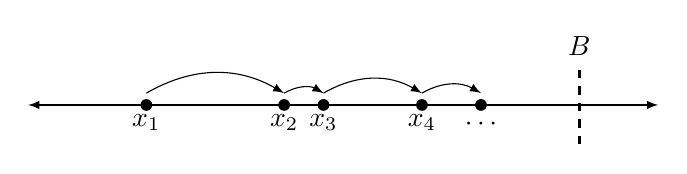
\begin{tikzpicture}[scale=1]
            \draw [<->, >=latex] (-4, 0) -- (4, 0);

            \node[below] at (-2.5, 0) {$x_1$};
            \node at (-2.5, 0) [circle, fill, inner sep = 1.5pt] {};

            \node[below] at (-0.75, 0) {$x_2$};
            \node at (-0.75, 0) [circle, fill, inner sep = 1.5pt] {};

            \node[below] at (-0.25, 0) {$x_3$};
            \node at (-0.25, 0) [circle, fill, inner sep = 1.5pt] {};

            \node[below] at (1, 0) {$x_4$};
            \node at (1, 0) [circle, fill, inner sep = 1.5pt] {};

            \node[below] at (1.75, -0.05) {$\cdots$};
            \node at (1.75, 0) [circle, fill, inner sep = 1.5pt] {};

            \draw [dashed, line width=1pt] (3, -0.5) -- (3, 0.5);
            \node[above] at (3, 0.5) {$B$};

            \draw [->, >=latex] (-2.5,   0.15) to[bend left] (-0.75,  0.15);
            \draw [->, >=latex] (-0.75,  0.15) to[bend left] (-0.25,  0.15);
            \draw [->, >=latex] (-0.25,  0.15) to[bend left] (1,      0.15);
            \draw [->, >=latex] (1,      0.15) to[bend left] (1.75,   0.15);
          \end{tikzpicture}
        \end{figure}

      \item The issue is that it is clearly not getting \textit{arbitrarily} closer to any bound. Any number $C$ bigger than $B$ will be an upper bound as well but it has no chance of being the limit because the distance will always be at least $C - B > 0$.

      \item The turning point of the proof is to realize that you want the \textit{smallest} upper bound you can get away with, otherwise known as the $\sup$.
        \begin{align*}
          \overline{x} \equiv \sup \Fset{x_m}
        \end{align*}

        Since $x_m$ is a bounded subset of $\mathbb{R}$, we know from class the $\sup$ exists.

      \item Now leverage the fact $\overline{x}$ is the \textit{smallest} upper bound. In particular, for \textit{any} $\widetilde{x} < \overline{x}$, there is some element of $x_m$ that is strictly greater than $\widetilde{x}$ (if not, then $\widetilde{x}$ is an upper bound of $\overline{x}$ that is smaller than $\overline{x}$, contradiction because $\overline{x}$ is the smallest upper bound).

        Formally, $\forall \widetilde{x} < \overline{x}$ there exists some $M$ s.t.
        \begin{align*}
          x_M > \widetilde{x}
        \end{align*}

        Let $\varepsilon \equiv \overline{x} - \widetilde{x}$, so $\forall \varepsilon > 0 ~~ \exists M$ s.t.
        \begin{align*}
          x_M > \overline{x} - \varepsilon
          \iff
          \varepsilon > \overline{x} - x_M = d(\overline{x}, x_M)
        \end{align*}

      \item This is very close to the definition of convergence! What is missing? Take any $m \ge M$; since $x_m$ is increasing, we know $x_m \ge x_M$. Therefore $\forall \varepsilon > 0$ we have
        \begin{align*}
          m \ge M
          \implies
          x_m \ge x_M
          \implies
          \overline{x} - x_m \le \overline{x} - x_M < \varepsilon
          \implies
          d(\overline{x}, x_m) < \varepsilon
        \end{align*}

        which means $x_m \to \overline{x}$ by definition.
      \end{itemize}

      There is a completely analogous proof for $(x_m)$ decreasing (or it would suffice to show $-x_m \to x \implies x_m$ converges). In general there is no need to do two different proofs when taking a shortcut would suffice; I only offer a different proofs below for illustrative purposes.

    \item Let us try a proof by contradiction to exhibit how one can use a theorem instead of the definition of convergence (though we will use other definitions). Let $(x_m)$ be decreasing.
    \begin{itemize}[label=$\circ$]
      \item Suppose $(x_m)$ does not converge. What do we know about sequences that do not converge?  A promising avenue is to consider the contrapositive of statements that give us convergent sequences. The one that will help us here is the fact that Cauchy sequences converge in $\mathbb{R}$.

      \item If the real sequence $(x_m)$ does not converge it is not Cauchy.

      \item The definition of Cauchy is that $\forall \varepsilon > 0 ~~ \exists M$ s.t. $\forall k, l \ge M$ we have $d(x_k, x_l) \le \varepsilon$.

      \item The negation of Cauchy is that $\exists \varepsilon > 0$ s.t. $\forall M ~~ \exists k, l \ge M$ s.t. $d(x_k, x_l) > \varepsilon$.

      \item The sequence is decreasing, so for such an $\varepsilon > 0$ and for $M_1 = 1$ we know $\exists k_1, l_1 \ge M_1$ s.t.
        \begin{align*}
          d(x_{k_1}, d_{l_1}) > \varepsilon
        \end{align*}

        Let us iterate, for $M_n > \max\set{k_{n - 1}, l_{ n -1}}$ we know $\exists k_n, l_n \ge M_n$ s.t.
        \begin{align*}
          d(x_{k_n}, x_{l_n}) > \varepsilon
        \end{align*}

      \item Intuitively, this means that we can always eventually find two elements of the sequence that are $\varepsilon$ way from each other. Hence there are infinitely many elements of the sequence with a distance of $\varepsilon$. However, $A$ is a lower bound, and $d(x_1, A)$ is finite because $x_1$ is a \textit{given number}.

        \begin{figure}[H]
          \centering
          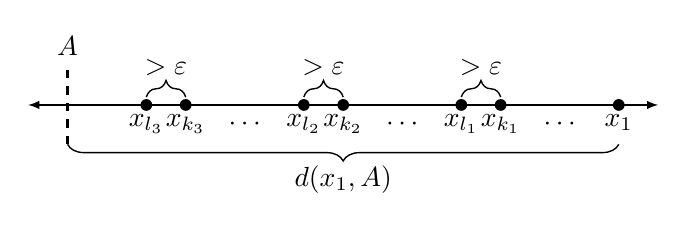
\begin{tikzpicture}[scale=1]
            \draw [<->, >=latex] (-4, 0) -- (4, 0);

            \node[below] at (-1.25, -0.05) {$\cdots$};
            \node[below] at (-2.5, 0) {$x_{l_3}$};
            \node at (-2.5, 0) [circle, fill, inner sep = 1.5pt] {};
            \node[below] at (-2, 0) {$x_{k_3}$};
            \node at (-2, 0) [circle, fill, inner sep = 1.5pt] {};
            \draw [
              decorate,
              decoration={brace, amplitude=6pt},
              xshift=0pt,
              yshift=0pt,
              line width=0.5pt
            ]
            (-2.5, 0.1) -- (-2, 0.1)
            node[above] at (-2.25, 0.25) {$> \varepsilon$};

            \node[below] at (0.75, -0.05) {$\cdots$};
            \node[below] at (-0.5, 0) {$x_{l_2}$};
            \node at (-0.5, 0) [circle, fill, inner sep = 1.5pt] {};
            \node[below] at (0, 0) {$x_{k_2}$};
            \node at (0, 0) [circle, fill, inner sep = 1.5pt] {};
            \draw [
              decorate,
              decoration={brace, amplitude=6pt},
              xshift=0pt,
              yshift=0pt,
              line width=0.5pt
            ]
            (-0.5, 0.1) -- (0, 0.1)
            node[above] at (-0.25, 0.25) {$> \varepsilon$};

            \node[below] at (2.75, -0.05) {$\cdots$};
            \node[below] at (1.5, 0) {$x_{l_1}$};
            \node at (1.5, 0) [circle, fill, inner sep = 1.5pt] {};
            \node[below] at (2, 0) {$x_{k_1}$};
            \node at (2, 0) [circle, fill, inner sep = 1.5pt] {};
            \draw [
              decorate,
              decoration={brace, amplitude=6pt},
              xshift=0pt,
              yshift=0pt,
              line width=0.5pt
            ]
            (1.5, 0.1) -- (2, 0.1)
            node[above] at (1.75, 0.25) {$> \varepsilon$};

            \node[below] at (3.5, 0) {$x_1$};
            \node at (3.5, 0) [circle, fill, inner sep = 1.5pt] {};

            \draw [dashed, line width=1pt] (-3.5, -0.5) -- (-3.5, 0.5);
            \node[above] at (-3.5, 0.5) {$A$};

            \draw [
              decorate,
              decoration={brace, amplitude=6pt},
              xshift=0pt,
              yshift=0pt,
              line width=0.5pt
            ]
            (3.5, -0.5) -- (-3.5, -0.5)
            node[below] at (0, -0.65) {$d(x_1, A)$};
          \end{tikzpicture}
        \end{figure}

        The sequence is decreasing, so there should be at most $(x_1 - A) / \varepsilon$ elements with a distance as big as $\varepsilon$, not infinitely many. How can we get the contradiction formally?

      \item WLOG suppose $x_{k_n} > x_{l_n}$ (note they cannot be equal at any $n$ or $d(x_{k_n}, x_{l_n})$ would be $0 < \varepsilon$).  This is WLOG because at any $n$ we can just denote the smaller element of the pair to be $x_{l_n}$. Hence
        \begin{align*}
          d(x_{k_n}, x_{l_n}) = x_{k_n} - x_{l_n} > \varepsilon
        \end{align*}

      \item Note $k_n, l_n \ge M_n > \max\set{k_{n - 1}, l_{n - 1}}$, \textit{both} $k_n, l_n$ are greater than \textit{either} $k_{n - 1}, l_{n - 1}$. Since $(x_m)$ is decreasing, $k_n >  l_{n - 1} \implies x_{k_n} \le x_{l_{n - 1}}$. Now pick any $n$:
        \begin{align*}
          x_{l_n} - A
          <
          x_{k_n} - A - \varepsilon
          \le
          x_{l_{n - 1}} - A - \varepsilon
          <
          x_{k_{n - 1}} - A - 2 \varepsilon
          <
          \ldots
          \le
          x_{k_1} - A - n \varepsilon
        \end{align*}

        We can see that
        \begin{align*}
          \dfrac{x_{l_1} - A}{\varepsilon} < n
          \implies
          x_{l_1} - A - n \varepsilon < 0
          \implies
          x_{l_n} - A < 0
        \end{align*}

        so $x_{l_n} < A$, meaning $A$ is not a lower bound, contradiction.

      \item Hence $(x_m)$ converges.
    \end{itemize}

  % \item The proof when $(x_m)$ is decreasing is completely analogous! So now we can see that all the work we did above will make this part easier. Here is the proof, abridged:
  %   \begin{itemize}[label=$\bullet$]
  %     \item Let $\underline{x} \equiv \inf \Fset{x_m}$; the $\inf$ is well-defined since $\Fset{x_m}$ is a  bounded subset of $\mathbb{R}$.
  %
  %     \item Take any $\varepsilon > 0$; by definition of the $\inf$ there exists some $M$ s.t.
  %       \begin{align*}
  %         x_M < \underline{x} + \varepsilon
  %       \end{align*}
  %
  %     \item Note $d(x_m, \underline{x}) = x_m - \underline{x}$ since $\underline{x} \le x_m$ for each $m$.
  %
  %     \item Finally, $x_m$ is decreasing, so for any $m \ge M$ we have
  %       \begin{align*}
  %         x_m \le x_M
  %         \implies
  %         d(x_m, \underline{x}) = x_m - \underline{x} \le x_M - \underline{x} < \varepsilon
  %       \end{align*}
  %
  %       completing the proof.
  %   \end{itemize}
\end{enumerate}

%----------------------------------------------------------------------
\end{document}
